\documentclass[a4paper,12pt]{extarticle}
\usepackage{geometry}
\usepackage[T1]{fontenc}
\usepackage[utf8]{inputenc}
\usepackage[english,russian]{babel}
\usepackage{mathptmx}
\usepackage{amsmath}
\usepackage{amsthm}
\usepackage{amssymb}
\usepackage{fancyhdr}
\usepackage{setspace}
\usepackage{graphicx}
\usepackage{caption}
\captionsetup{labelsep=endash, justification=raggedright, singlelinecheck=false}
\usepackage{colortbl}
\usepackage{tikz}
\usepackage{pgf}
\usepackage{subcaption}
\usepackage{listings}
\usepackage{indentfirst}
\usepackage[
backend=biber,
style=numeric,
maxbibnames=99
]{biblatex}
\addbibresource{refs.bib}
\usepackage[colorlinks,citecolor=blue,linkcolor=blue,bookmarks=false,hypertexnames=true, urlcolor=blue]{hyperref}
\usepackage{indentfirst}
\usepackage{mathtools}
\usepackage{booktabs}
\usepackage[flushleft]{threeparttable}
\usepackage{tablefootnote}
\usepackage{chngcntr} % нумерация графиков и таблиц по секциям
\counterwithin{table}{section}
\counterwithin{figure}{section}
\makeatletter
% \renewcommand{@biblabel}[1]{1.} % Заменяем библиографию с квадратных скобок на точку:
\makeatother
\geometry{left=2.5cm}% левое поле
\geometry{right=1.0cm}% правое поле
\geometry{top=2.0cm}% верхнее поле
\geometry{bottom=2.0cm}% нижнее поле
\setlength{\parindent}{1.25cm}
\renewcommand{\baselinestretch}{1.5} % междустрочный интервал
\newcommand{\bibref}[3]{\hyperlink{1}{2 (3)}} % biblabel, authors, year
\addto\captionsrussian{\def\refname{Список литературы (или источников)}}
\renewcommand{\theenumi}{\arabic{enumi}}% Меняем везде перечисления на цифра.цифра
\renewcommand{\labelenumi}{\arabic{enumi}}% Меняем везде перечисления на цифра.цифра
\renewcommand{\theenumii}{.\arabic{enumii}}% Меняем везде перечисления на цифра.цифра
\renewcommand{\labelenumii}{\arabic{enumi}.\arabic{enumii}.}% Меняем везде перечисления на цифра.цифра
\renewcommand{\theenumiii}{.\arabic{enumiii}}% Меняем везде перечисления на цифра.цифра
\renewcommand{\labelenumiii}{\arabic{enumi}.\arabic{enumii}.\arabic{enumiii}.}% Меняем везде перечисления на цифра.цифра
\begin{document}
\begin{titlepage}
\begin{center}
    % Добавляем вертикальный отступ сверху, чтобы название не было прижато к краю
    \vspace*{6cm} 
    
    % НАЗВАНИЕ РАБОТЫ
    {\Huge\bfseries Прогнозирование за горизонтом прогнозирования: прогнозирование хаотических временных рядов\par}
    
    \vspace{4cm} % Отступ между названием и ключевыми словами
    
    % КЛЮЧЕВЫЕ СЛОВА
    \begin{minipage}{0.8\textwidth}
        \large
        \textbf{Ключевые слова:} Прогнозирование хаотических временных рядов, система Лоренца, расширение обучающей выборки, метод мотивов, непрогнозируемые точки, 
        кластеризация данных, дефицит данных.
    \end{minipage}

\end{center}

\vfill % Заполняет оставшееся пространство, отодвигая все, что ниже, к низу страницы
% Год и город убраны по требованиям анонимизации

\end{titlepage}% это титульный лист выберите подходящий вам из имеющихся в проекте вариантов (kr курсовая работа у 3 курса, vkr выпускная квалификационная работа у 4 курса)
\newpage
\section*{Аннотация}
Данная работа посвящена исследованию улучшения точности прогнозирования хаотических временных 
рядов путем расширения обучающей выборки данными из схожих динамических систем. В ходе исследования
 на данных системы Лоренца было установлено, что не всякая формально близкая система является
  полезным донором данных, и их неверный выбор может ухудшить качество прогноза. Для решения 
  этой проблемы был разработан и валидирован новый критерий для априорного отбора совместимых
   рядов, основанный на сравнении их статистических инвариантов. Эксперименты подтвердили, что
    использование этой метрики позволяет целенаправленно улучшать прогноз, добиваясь значительного
     сокращения непрогнозируемых точек при сохранении высокой точности.
  \subsection*{Ключевые слова}
Прогнозирование хаотических временных рядов, система Лоренца,
расширение обучающей выборки, метод мотивов, непрогнозируемые точки

\newpage
\tableofcontents
\newpage
\section{Введение}
Прогнозирование хаотических временных рядов фундаментально ограничено
 горизонтом прогнозирования, за пределами которого чувствительность
  к начальным условиям приводит к экспоненциальному росту ошибки. \cite{MalinetskiyPotapov2002, Gilmore1984}
  Традиционные итеративные методы, предсказывающие на один шаг вперед,
   быстро накапливают эту ошибку, что делает их неэффективными для долгосрочных
    прогнозов. Альтернативой служат методы, основанные на поиске характерных
    последовательностей (мотивов), которые реконструируют динамику системы в
    фазовом пространстве и ищут в прошлом аналоги текущего состояния.

Однако практическая эффективность таких методов ограничивается проблемой, известной как проклятие размерности.
. Для надежной реконструкции аттрактора и нахождения статистически
 значимого числа мотивов требуется объем данных $N$, экспоненциально растущий
  с размерностью вложения $d$. Даже в идеализированной ситуации, когда аттрактор
   представляет собой $d$-мерный куб со стороной $a$, для его адекватного заполнения
    необходимо $N \sim \frac{a^d}{(0.1a)^d} = 10^d$ точек. Для реальных систем,
    динамика которых разворачивается на фрактальных аттракторах, ситуация усугубляется:
     $N > N_0 \cdot 10^d$, где множитель $N_0 \sim \epsilon_{fr}^{-d}$ зависит
     от масштаба фрактальности $\epsilon_{fr}$. На практике, например для финансовых
      данных, это может потребовать порядка $10^9$ наблюдений.

Эта проблема усугубляется требованием стационарности данных. Динамическая система,
генерирующая временной ряд, может изменять свои свойства с течением времени, что
делает старые участки ряда нерелевантными для описания текущей динамики. Таким
образом, возникает фундаментальное противоречие: для преодоления проклятия размерности
 требуется огромный объем данных, но требование стационарности жестко ограничивает
 длину выборки, которую можно считать однородной и пригодной для обучения.

Предлагаемый в данной работе подход является попыткой разрешить это противоречие.
 Мы ставим ключевой исследовательский вопрос: \textbf{возможно ли компенсировать
  дефицит данных в целевом временном ряду за счет привлечения выборок из других,
   формально независимых, но схожих по поведению процессов?} Наша центральная гипотеза
    состоит в том, что различные, но связанные процессы могут разделять общий
     словарь локальных поведенческих паттернов (мотивов). В этом случае можно
     объединить несколько более коротких, но стационарных выборок из разных источников,
      чтобы сформировать одну, достаточно богатую для обучения. Статистическая выгода
      от создания такой разнообразной библиотеки мотивов может перевесить шум, вносимый
      данными из неидентичного источника.

Для строгой проверки этой гипотезы в качестве контролируемой среды была
 выбрана система Лоренца, позволяющая точно дозировать степень несхожести между рядами.
В рамках исследования была поставлена задача количественно оценить влияние
 расширения обучающей выборки данными из схожих динамических систем на точность
  прогноза (RMSE, MAPE) и долю непрогнозируемых точек. Для этого исследовалась 
  зависимость качества прогноза от величины расхождения в управляющих параметрах 
  между целевой и вспомогательной системами, чтобы определить границы применимости 
  подхода.  Ключевой и синтезирующей задачей работы стала разработка и 
  экспериментальная апробация метрики для априорной оценки прогностической 
  совместимости временных рядов, позволяющей целенаправленно отбирать наиболее
   эффективные ряды-доноры для аугментации.



\section{Обзор литературы}

Основой для настоящего исследования служат работы В.А. Громова и Ф.С. Баранова  \cite{GromovBaranov2023}
, в которых предложен метод прогнозирования хаотических временных рядов,
 основанный на поиске характерных последовательностей (мотивов).
  Суть подхода заключается в реконструкции фазового пространства
   системы по наблюдаемому временному ряду и последующей кластеризации
   векторов состояний для выявления повторяющихся паттернов динамики.

Ключевой особенностью метода является использование множества мотивов,
что порождает набор возможных прогнозных значений для каждой точки.
 Для получения единого прогноза (унификации) в предыдущих работах
  рассматривались различные подходы, включая вычисление среднего
   значения, применение взвешенного усреднения (в зависимости от длины прогноза или расстояния
    до центра кластера) и выбор центра наиболее крупного кластера из возможных прогнозов.

Важнейшим аспектом, отличающим данный подход, является концепция
непрогнозируемых точек. Она позволяет алгоритму оценивать собственную уверенность
 и воздерживаться от прогноза в ситуациях высокой неопределенности,
 что повышает надежность модели. Для идентификации таких точек применялись
 как статистические критерии (энтропия множества прогнозных значений, его
 мультимодальность, ширина интерквантильного размаха), так и более сложные
 классификаторы на основе методов машинного обучения, включая логистическую регрессию,
  метод опорных векторов (SVM), деревья решений, k-NN, многослойные перцептроны (MLP) и их ансамбли.\cite{Wang2019}

Исследования показали высокую эффективность метода: алгоритм демонстрировал
практически постоянную ошибку прогноза (MAE, RMSE) даже при увеличении
горизонта до 100 шагов вперед, что достигалось за счет экспоненциального
 роста числа точек, классифицируемых как непрогнозируемые. Особое значение
  для настоящей работы имеет исследование  \cite{Gromov2021}, в котором изучалось влияние

  размера обучающей выборки на точность. Было установлено, что при увеличении о
  бъема данных из исходного ряда ошибка прогноза убывала логарифмически. Однако
  вопрос о том, можно ли компенсировать недостаток данных за счет добавления
  выборок из других, но схожих по динамике систем, оставался открытым.
 Данная работа направлена на исследование именно этой возможности.

\subsection{Формальная Постановка задачи}

Данная работа посвящена задаче многошагового прогнозирования хаотических
 временных рядов в условиях ограниченности данных. Мы рассматриваем ситуацию,
  когда доступно множество временных рядов $\mathcal{Y} = \{Y^{(0)}, Y^{(1)},
   \dots, Y^{(M)}\}$, где $Y^{(0)}$ является \textit{целевым} рядом, для которого
    необходимо построить прогноз, а $Y^{(1)}, \dots, Y^{(M)}$ — \textit{вспомогательными} рядами.
     Предполагается, что вспомогательные ряды порождены динамическими системами,
      схожими с целевой, но не обязательно идентичными ей.

Все временные ряды $Y^{(m)} = \{y_0^{(m)}, y_1^{(m)}, \dots\} \in \mathcal{Y}$ удовлетворяют следующим допущениям:
\begin{enumerate}
    \item В каждом ряду завершились все переходные процессы, и наблюдаемая
    динамика происходит в окрестности странного аттрактора.
    \item Каждый ряд удовлетворяет условиям теоремы Такенса\cite{Takens1981}, что делает
    возможным корректную реконструкцию аттрактора по одномерным наблюдениям.
\end{enumerate}

Для постановки задачи прогнозирования и его последующей оценки данные разделяются
 следующим образом. Целевой ряд $Y^{(0)}$ разбивается на две непересекающиеся части:
  обучающую (наблюдаемую) выборку $Y_1^{(0)} = \{y_0^{(0)}, \dots, y_t^{(0)}\}$ и
   тестовую выборку $Y_2^{(0)} = \{y_{t+1}^{(0)}, y_{t+2}^{(0)}, \dots\}$, на которой
    производится оценка качества прогноза. Вспомогательные ряды $Y^{(1)}, \dots, Y^{(M)}$
     используются для обучения целиком. Таким образом, полное обучающее множество
     $\mathcal{D}_{\text{train}}$ определяется как объединение наблюдаемой части
      целевого ряда и всех вспомогательных рядов:
\[
\mathcal{D}_{\text{train}} = \{Y_1^{(0)}, Y^{(1)}, \dots, Y^{(M)}\}.
\]

Ключевой особенностью предлагаемого подхода является то, что для каждой
 прогнозируемой точки $y_{t+h}^{(0)}$ из тестовой выборки $Y_2^{(0)}$ алгоритм
  генерирует не одно-единственное значение, а \textit{множество возможных предсказаний}
   $\hat{S}_{t+h}$. Это множество формируется функцией $f_h$, которая использует
   как историю целевого ряда, так и всю информацию из полного обучающего множества $\mathcal{D}_{\text{train}}$:
\[
\hat{S}_{t+h} = f_h\left(\{y_t^{(0)}, y_{t-1}^{(0)}, \dots, y_{t-s+1}^{(0)}\}; \mathcal{D}_{\text{train}}\right),
\]
где $s$ — параметр, определяющий длину используемой истории.

Над множеством $\hat{S}_{t+h}$ определены два оператора. Первый оператор,
 $\zeta(\cdot)$, проверяет, является ли позиция $t+h$ прогнозируемой на
 основе анализа распределения значений в $\hat{S}_{t+h}$:
\begin{equation}
\zeta(\hat{S}_{t+h}) =
\begin{cases}
1, & \text{если позиция прогнозируема,} \\
0, & \text{в противном случае.}
\end{cases}
\end{equation}
Второй оператор, $g(\cdot)$, вычисляет единое прогнозное значение
(Unified Predicted Value, UPV) для прогнозируемой позиции:
\begin{equation}
\hat{y}_{t+h} = g(\hat{S}_{t+h}).
\end{equation}

С использованием этих операторов задача многошагового прогнозирования
 формулируется как двухкритериальная оптимизация. Необходимо одновременно
 минимизировать два функционала, вычисляемых на тестовой выборке $Y_2^{(0)}$:
\begin{enumerate}
    \item \textbf{Функционал числа непрогнозируемых точек ($I_1$):}
    \begin{equation}
    I_1 = \sum_{y_{t+h}^{(0)} \in Y_2^{(0)}} \left( 1 - \zeta(\hat{S}_{t+h}) \right) \to \min.
    \end{equation}

\item \textbf{Функционал ошибки на прогнозируемых точках ($I_2$):}
    \begin{equation}
    I_2 = \frac{1}{|Y_{\text{pred}}^{(0)}|} \sum_{y_{t+h}^{(0)} \in Y_{\text{pred}}^{(0)}} L(\hat{y}_{t+h}, y_{t+h}^{(0)}) \to \min,
    \end{equation},где $L(\hat{y}, y)$~--- функция потерь.
\end{enumerate}
где $Y_{\text{pred}}^{(0)} \subseteq Y_2^{(0)}$ — подмножество точек, для
 которых $\zeta(\hat{S}_{t+h}) = 1$. Настоящая работа направлена на решение
  этой двухкритериальной задачи путем эффективного использования расширенного
   обучающего множества $\mathcal{D}_{\text{train}}$.
\subsection{Генерация обобщенных z-векторов и формирование выборок}

Для эффективного захвата нелокальных во времени корреляций, присущих хаотическим системам,
 мы используем концепцию обобщенных z-векторов, построенных на основе предопределенных шаблонов.

Шаблоном называется целочисленный вектор $\boldsymbol{k} = (k_1, k_2, \dots, k_{L-1})$,
 где $L$ — длина z-вектора (число используемых наблюдений), а $1 \le k_j \le K_{\max}$ — шаг между $j$-м и $(j+1)$-м наблюдением в векторе.

Для каждого временного ряда $Y^{(m)} \in \mathcal{D}_{\text{train}}$ и каждого шаблона
 $\boldsymbol{k}$ из множества всех комбинаторно возможных шаблонов $\aleph(L, K_{\max})$
  генерируется собственная выборка обобщенных z-векторов. Z-вектор в момент времени $t$ определяется как:
\[
\mathbf{z}_{t}^{(m, \boldsymbol{k})} = \bigl(y^{(m)}_t,\ y^{(m)}_{t+k_1},\ y^{(m)}_{t+k_1+k_2},\ \dots,\ y^{(m)}_{t + \sum_{j=1}^{L-1} k_j}\bigr).
\]


Ключевым шагом нашего подхода является \textbf{объединение} всех выборок, сгенерированных
 по одному и тому же шаблону $\boldsymbol{k}$, но из разных временных рядов, в единое множество:
\[
\mathcal{Z}^{(\boldsymbol{k})} = \bigcup_{m=0}^{M} \left\{ \mathbf{z}_{t}^{(m, \boldsymbol{k})} \right\}_{t}.
\]
Таким образом, для каждого шаблона $\boldsymbol{k}$ формируется одна, но значительно
 более плотная и разнообразная обучающая выборка $\mathcal{Z}^{(\boldsymbol{k})}$,
  аккумулирующая информацию о динамике всего семейства систем.

\subsection{Кластеризация и формирование библиотеки мотивов}

Каждая объединенная выборка $\mathcal{Z}^{(\boldsymbol{k})}$ кластеризуется отдельно
 для выявления типичных, повторяющихся паттернов поведения. Центры полученных кластеров
  интерпретируются как \textit{мотивы}.
\textbf{Мотивом}, соответствующим шаблону $\boldsymbol{k}$,
 называется вектор $C_{\boldsymbol{k}} = (\eta_{\boldsymbol{k},1},
 \eta_{\boldsymbol{k},2}, \dots, \eta_{\boldsymbol{k},L})$, являющийся
 центром кластера в пространстве z-векторов $\mathcal{Z}^{(\boldsymbol{k})}$.

Множество всех мотивов, полученных для шаблона $\boldsymbol{k}$,
обозначается $\Psi_{\boldsymbol{k}}$. Полная \textit{библиотека мотивов}
 $\Psi$ представляет собой множество пар (шаблон,мотивы) для всех возможных
  шаблонов и определяется следующим образом:
\[
\Psi = \left\{ (\boldsymbol{k}, \Psi_{\boldsymbol{k}}) \mid \boldsymbol{k}
\in \aleph(L, K_{\max}) \right\}.
\]
Эта библиотека кодирует обобщенную динамику, свойственную всему классу рассматриваемых
 систем, и служит основой для построения прогнозов.

\subsection{Формирование множества возможных предсказаний}

Прогнозирование точки $y_{t+h}^{(0)}$ целевого ряда $Y^{(0)}$
 выполняется путем поиска в библиотеке $\Psi$ мотивов, чье начало
  соответствует недавней истории целевого ряда. Процесс состоит из следующих шагов:
\begin{enumerate}
    \item Для каждого шаблона $\boldsymbol{k}$ из истории целевого
     ряда $\{y_{t}^{(0)}, y_{t-1}^{(0)}, \dots\}$ формируется \textit{запрашивающий вектор}
      $C_{\text{query}}^{(\boldsymbol{k})}$, состоящий из $L-1$ элементов
       и структурно идентичный усеченному мотиву.

    \item Этот вектор сравнивается со всеми усеченными мотивами $C_{\boldsymbol{k},
     \text{trunc}} = (\eta_{\boldsymbol{k},1}, \dots, \eta_{\boldsymbol{k}, L-1})$
     из множества $\Psi_{\boldsymbol{k}}$.

    \item Если евклидово расстояние $\rho(C_{\text{query}}^{(\boldsymbol{k})},
     C_{\boldsymbol{k}, \text{trunc}})$ меньше заданного порога $\varepsilon$,
      то последний элемент соответствующего полного мотива, $\eta_{\boldsymbol{k},L}$,
       считается возможным предсказанием. Множество таких предсказаний для одного шаблона
       обозначается $\hat{S}_{t+h}^{(\boldsymbol{k})}$.

    \item Итоговое \textit{множество возможных предсказаний} $\hat{S}_{t+h}$ для
     точки $y_{t+h}^{(0)}$ является объединением предсказаний, полученных по всем шаблонам:
    \[
    \hat{S}_{t+h} = \bigcup_{\boldsymbol{k} \in \aleph(L, K_{\max})} \hat{S}_{t+h}^{(\boldsymbol{k})}.
    \]
\end{enumerate}

Полученное множество $\hat{S}_{t+h}$ является эмпирическим распределением и служит
 основой для последующего анализа. Если распределение значений в $\hat{S}_{t+h}$
  является плотным и унимодальным, точка считается прогнозируемой, и для нее
  вычисляется единое прогнозное значение (UPV). Если же распределение разреженное,
   мультимодальное или равномерное, точка классифицируется как непрогнозируемая.
    Детальное описание методов классификации и вычисления UPV представлено в следующем разделе.
\section{Вычисление прогноза и идентификация непрогнозируемых точек}

Центральным этапом предлагаемого подхода является анализ эмпирического распределения
 $\hat{S}_{t+h}$, полученного для каждой прогнозируемой точки $y_{t+h}^{(0)}$. Этот
  анализ решает две взаимосвязанные задачи: определение, является ли точка прогнозируемой,
   и, если да, вычисление для нее единого прогнозного значения (UPV). В данной работе обе
   задачи решаются с помощью единого инструмента~--- кластеризации множества $\hat{S}_{t+h}$ алгоритмом DBSCAN. \cite{Aggarwal2013}

\subsection{Интегрированный подход на основе кластеризации}

Для каждого непустого множества $\hat{S}_{t+h}$ выполняется процедура кластеризации,
 которая разбивает его на $N_c$ кластеров $\{Q_1, Q_2, \dots, Q_{N_c}\}$. Пусть $|Q_j|$~--- число
  элементов (мощность) $j$-го кластера. Кластеры упорядочиваются по убыванию мощности:
   $|Q_1| \ge |Q_2| \ge \dots \ge |Q_{N_c}|$.

\textbf{Идентификация непрогнозируемых точек} производится на основе анализа этой
кластерной структуры. Точка $y_{t+h}^{(0)}$ считается \textit{прогнозируемой} тогда
 и только тогда, когда в множестве ее предсказаний $\hat{S}_{t+h}$ существует один
 доминирующий кластер. Формально, это условие выражается следующим образом:
\[
\zeta(\hat{S}_{t+h}) =
\begin{cases}
1, & \text{если } |Q_1| \ge \alpha \cdot |Q_2| \text{ (для } N_c > 1\text{) или } N_c = 1, \\
0, & \text{в противном случае,}
\end{cases}
\]
где $\alpha > 1$~--- гиперпараметр, задающий требуемую степень доминирования
 крупнейшего кластера. Если самый большой кластер не превосходит по размеру
 второй по величине кластер как минимум в $\alpha$ раз, это свидетельствует о
 наличии нескольких конкурирующих, равновероятных сценариев будущего, что делает
  прогноз ненадежным. В этом случае точка классифицируется как \textit{непрогнозируемая}.
   Если множество $\hat{S}_{t+h}$ пусто, точка также считается непрогнозируемой.

\textbf{Вычисление единого прогнозного значения (UPV)} производится только для
 точек, классифицированных как прогнозируемые ($\zeta(\hat{S}_{t+h})=1$). В качестве итогового прогноза $\hat{y}_{t+h}$ принимается среднее арифметическое значение элементов, входящих в состав крупнейшего (доминирующего) кластера $Q_1$:
\[
\hat{y}_{t+h} = \frac{1}{|Q_1|} \sum_{\hat{y} \in Q_1} \hat{y}.
\]
Такой подход позволяет отфильтровать шумовые или менее согласованные группы
предсказаний и основывать прогноз на наиболее консенсусном и статистически значимом сценарии.

\subsection{"Демон": идеальный классификатор}

Для оценки качества предложенного метода идентификации непрогнозируемых точек и
определения теоретических пределов точности прогноза в работе используется
контрольный или идеальный метод. Этот метод предполагает наличие \textit{a priori}
 информации об истинном значении $y_{t+h}^{(0)}$ на этапе анализа.

В рамках этого подхода точка $y_{t+h}^{(0)}$ считается \textit{непрогнозируемой},
 если ошибка наилучшего возможного прогноза из множества $\hat{S}_{t+h}$ превышает заданный порог $\delta$:
\[
\zeta_{\text{ideal}}(\hat{S}_{t+h}) =
\begin{cases}
0, & \text{если } \min_{\hat{y} \in \hat{S}_{t+h}} |\hat{y} - y_{t+h}^{(0)}| > \delta, \\
1, & \text{в противном случае.}
\end{cases}
\]
В экспериментах использовалось значение $\delta = 0.05$. Этот метод,
 очевидно, не может быть применен на практике, но он позволяет установить ground-truth
  разметку непрогнозируемых точек и служит эталоном (верхней границей качества),
   с которым сравниваются результаты основного, практического метода.
\subsection{Алгоритм кластеризации для выявления мотивов}

Для выявления типичных, повторяющихся паттернов (мотивов) в каждой
объединенной выборке z-векторов $\mathcal{Z}^{(\boldsymbol{k})}$ применяется
алгоритм кластеризации, предложенный Лапко и Ченцовым на основе идей
Уишарта \cite{GromovBaranov2023}.

Ключевая идея метода заключается в непараметрической оценке плотности
распределения данных в многомерном пространстве. Алгоритм идентифицирует
плотные скопления точек (будущие кластеры) и определяет их границы,
что делает его эффективным для поиска структур произвольной формы
в фазовом пространстве, характерных для аттракторов динамических систем.

В результате работы алгоритма для каждой выборки $\mathcal{Z}^{(\boldsymbol{k})}$
формируется набор устойчивых кластеров. Центроиды этих кластеров
и принимаются в качестве искомых \textbf{мотивов}, которые затем используются
для построения библиотеки $\Psi$.
\section{Изучение системы Лоренца}

В качестве исследуемого ряда был выбран ряд Лоренца, который обладает
 фрактальной размерностью около 2. Основной ряд \(Y\) получен при стандартных
  параметрах: \(r = 28\), \(\sigma = 10\), \(b = 8/3\) путем использования стандартных методов \cite{Balashova1991}.
   Поведение системы
   Лоренца существенно зависит от значения параметра \(r\),что детально описано в
   работах \cite{KaplanYorke1979, Hateley2016}. Были обнаружены следующие характерные режимы:
\begin{enumerate}
    \item При \(r < 1\): система имеет единственную стационарную точку (0,0,0).
    \item При \(1 < r < 13.926\): появляются три стационарные точки.
    \item При \(r \approx 13.926\): возникают гомоклинические орбиты.
    \item При \(13.926 < r < 24.06\): наблюдается метастабильный хаос, хаотическое
     множество растёт, оставаясь неустойчивым и непритягивающим.
    \item При \(24.06 < r < 24.74\): аттрактор становится притягивающим, сохраняя две устойчивые точки.
    \item При \(r > 24.74\): формируется единственный глобальный странный аттрактор.
    \item При \(r > 50\): появляются устойчивые орбиты.
    \item При \(144 < r < 167\): система демонстрирует две периодические орбиты.
    \item При \(r > 167\): возникает прерывистый хаос с чередованием хаотических и периодических режимов.
\end{enumerate}

\subsection{Визуальный анализ и характеристика данных}

При работе с хаотическими системами необходимо четко разделять два
типа различий, возникающих при изменении управляющих параметров.
Качественные изменения, происходящие в точках бифуркации.
     В этих точках происходит фундаментальная перестройка динамики системы, и форма (топология) аттрактора кардинально меняется, например, хаотический аттрактор может смениться устойчивой периодической орбитой.
Количественные изменения, наблюдаемые между точками
     бифуркаций. В этом случае аттрактор сохраняет свою топологическую структуру,
      однако меняются его метрические свойства.

На Рисунке \ref{fig:lorenz_comparison} представлены участки траекторий, иллюстрирующие
именно количественные различия. Поскольку все выбранные для эксперимента значения
параметра \(r\) находятся в зоне устойчивого хаоса, форма аттрактора остается неизменной.

\begin{figure}[htbp]
    \centering
    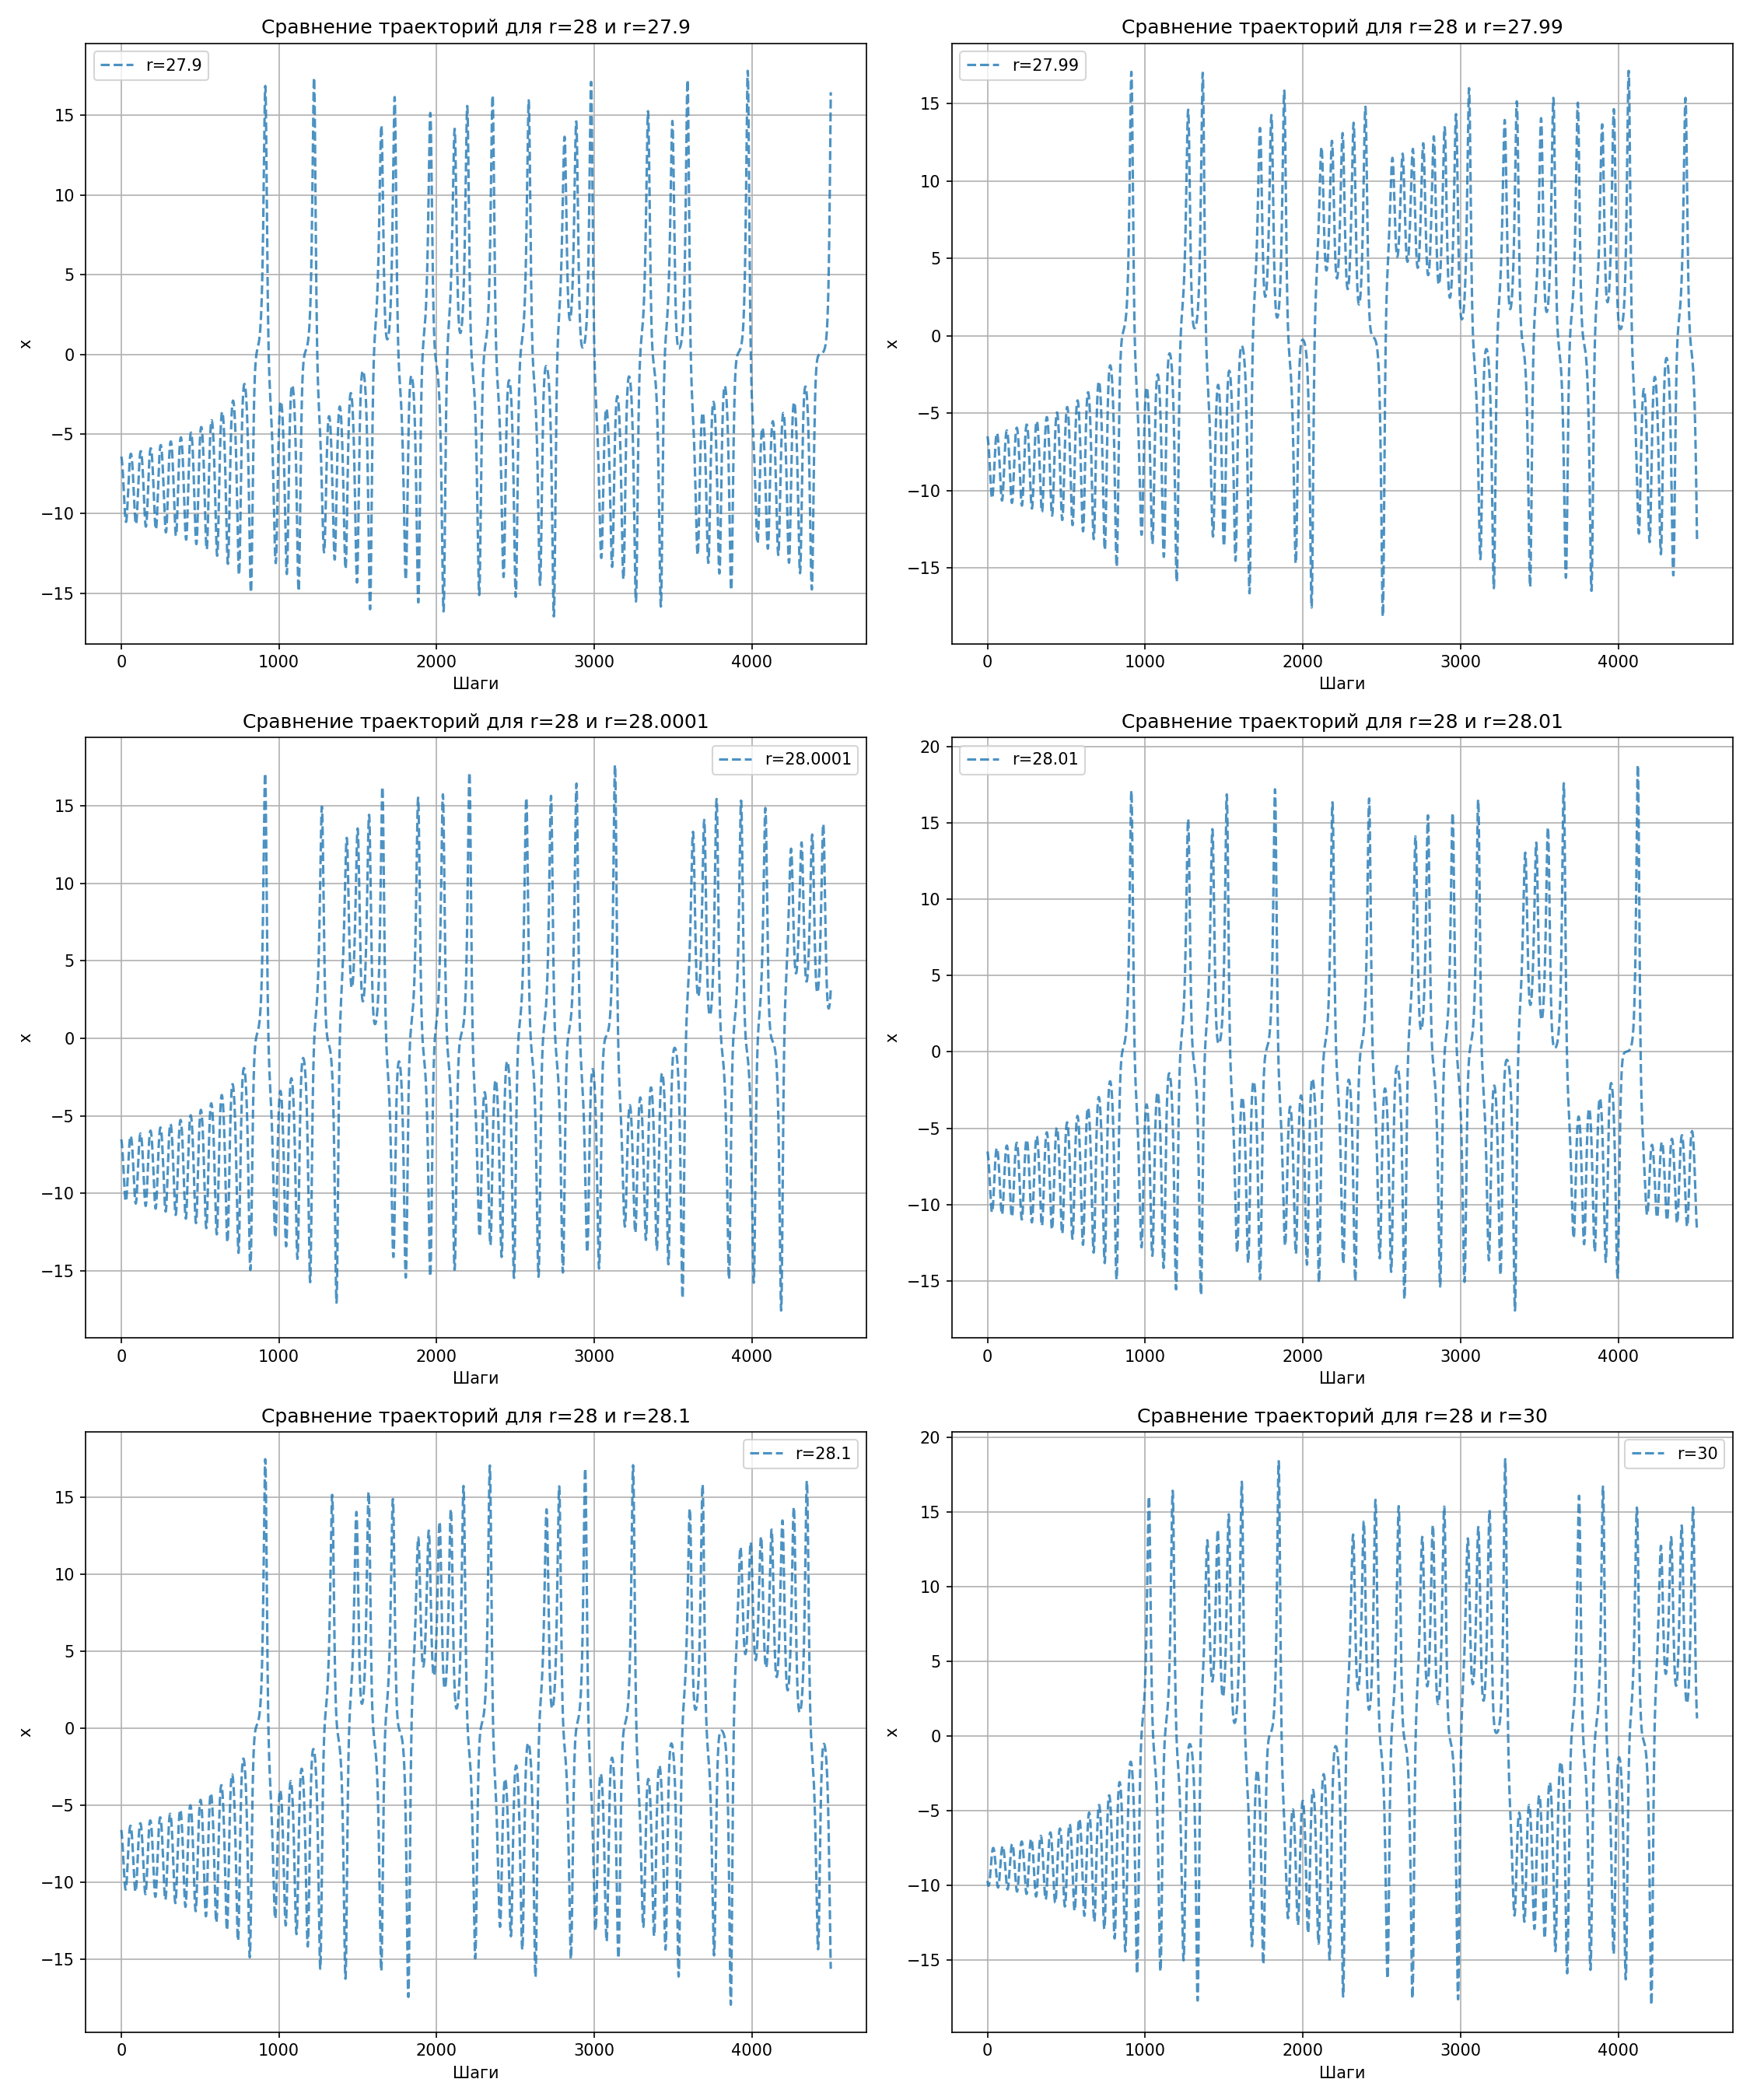
\includegraphics[width=\textwidth]{../dtw/rows.png}
    \caption{Сравнение участков траекторий системы Лоренца. Все представленные ряды находятся в области одного и того же странного аттрактора, поэтому его топологическая форма сохраняется. Однако визуально заметно, что при большем отклонении параметра \(r\) от базового значения \(r=28\), расхождение траекторий становится более быстрым и выраженным.}
    \label{fig:lorenz_comparison}
\end{figure}

Также были подсчитаны метрики,которые проверяли количественную схожесть рядов:DTW и корреляция Пирсона.
\begin{table}[htbp]
\centering
\caption{Сравнение метрик схожести для временных рядов аттрактора Лоренца при разных значениях параметра r (эталон r=28).}
\label{tab:lorenz_metrics}
% Добавляем вертикальные линии |
\begin{tabular}{|r|r|r|r|r|}
\hline % Верхняя горизонтальная линия
r Value & DTW Distance & Euclidean Distance & Pearson Correlation & Spearman Correlation \\
\hline % Линия под заголовком
28.0001 & 16386.4172 & 959.5454 & 0.2574 & 0.2819 \\
\hline % Линия после каждой строки
27.9900 & 16994.6190 & 1045.5196 & 0.1277 & 0.1439 \\
\hline
28.0100 & 18952.6397 & 1042.8613 & 0.1094 & 0.1254 \\
\hline
28.1000 & 17823.6581 & 1009.5965 & 0.1885 & 0.2159 \\
\hline
27.9000 & 19479.5353 & 1101.3690 & -0.0099 & 0.0153 \\
\hline
30.0000 & 20504.8125 & 1095.1419 & 0.0933 & 0.1106 \\
\hline
31.0000 & 20146.6934 & 1079.9026 & 0.1104 & 0.1290 \\
\hline
32.0000 & 18226.2998 & 1143.9155 & 0.0129 & 0.0289 \\
\hline
33.0000 & 18633.1070 & 1095.9076 & 0.1271 & 0.1406 \\
\hline
34.0000 & 20951.9940 & 1157.6998 & 0.0485 & 0.0536 \\
\hline
35.0000 & 22030.5267 & 1157.6071 & 0.0622 & 0.0731 \\
\hline
36.0000 & 25929.7317 & 1222.5457 & -0.0184 & -0.0067 \\
\hline
37.0000 & 24355.9578 & 1236.8270 & -0.0242 & -0.0232 \\
\hline
38.0000 & 27063.9970 & 1208.5813 & 0.0638 & 0.0723 \\
\hline
39.0000 & 26136.9308 & 1173.3409 & 0.1090 & 0.1124 \\
\hline % Нижняя горизонтальная линия
\end{tabular}
\end{table}

Предварительный анализ как визуальных (Рисунок~\ref{fig:lorenz_comparison}),
 так и количественных (Таблица~\ref{tab:lorenz_metrics}) данных, казалось
  бы, дает однозначный ответ на вопрос о выборе наилучшего вспомогательного
   ряда. Визуально, траектория для $r=28.0001$ практически совпадает с эталонной
    ($r=28$) на протяжении почти 2000 шагов. Это наблюдение находит свое полное
     подтверждение в количественных метриках: данный ряд демонстрирует минимальное
      расстояние DTW и максимальную корреляцию, что делает его интуитивно наиболее
      предпочтительным кандидатом для расширения обучающей выборки.

Тем не менее, эта предварительная оценка, базирующаяся на глобальных метриках, оказывается обманчивой. Дальнейший анализ покажет, что ряд с параметром 
r=28.0001
, несмотря на его кажущееся превосходство, является неэффективным для аугментации. Напротив, ряд при *исходного*
r=27.99
, формально менее схожий, демонстрирует значительную прогностическую ценность, порой превосходящую даже эффект от добавления данных из самого целевого процесса.
Этот парадокс выявляет ключевое методологическое ограничение: метрики глобального характера (DTW, корреляция) не способны адекватно оценить пригодность ряда для методов, основанных на локальных паттернах. Успех используемого алгоритма прогнозирования определяется не интегральным сходством траекторий, а степенью пересечения их «словарей» локальных мотивов. Таким образом, глобальная когерентность не является достаточным условием для локальной совместимости динамик.
В свете этого, данные из Таблицы~\ref{tab:lorenz_metrics} и Рисунка~\ref{fig:lorenz_comparison} следует интерпретировать как демонстрацию неадекватности общепринятых подходов к сравнению рядов для решения поставленной задачи. Они доказывают, что прогностическая совместимость — это сложное, эмерджентное свойство системы, которое не может быть оценено простыми метриками и требует непосредственной экспериментальной проверки в рамках используемой модели прогнозирования.

\section{Экспериментальное исследование}

\subsection{Влияние аугментации на качество прогноза}
\subsubsection{Описание эксперимента}
Основной целью данного эксперимента являлась количественная оценка влияния размера и
состава обучающей выборки на качество многошагового прогнозирования. Экспериментальная
 установка была спроектирована для систематического исследования эффекта аугментаци
 и данных как из самого целевого процесса, так и из внешних, но схожих по динамике, систем.

В качестве целевого временного ряда $Y^{(0)}$ использовалась первая координата
 системы Лоренца, сгенерированная при канонических параметрах ($\sigma = 10$, $r = 28$, $b = 8/3$).
 Исходная обучающая выборка $Y_1^{(0)}$ состояла из 10 000 наблюдений. Для каждого из исследуемых
  вспомогательных рядов $Y^{(m)}$, сгенерированных с параметром $r$, незначительно отличающимся от
   базового, проводилась следующая итеративная процедура: к исходной выборке $Y_1^{(0)}$
   последовательно добавлялись сегменты данных из $Y^{(m)}$ до тех пор, пока общий размер
   объединенной выборки $\mathcal{D}_{\text{train}}$ не достигал 40 000 точек. Контрольный
   случай представлял собой аналогичное увеличение объема данных, но с использованием наблюдений
    из самого целевого ряда (т.е. $Y_1^{(0)}$ расширялся до 40 000 точек без привлечения внешних данных).

На каждом шаге увеличения размера выборки для полученного обучающего
 множества $\mathcal{D}_{\text{train}}$ выполнялось прогнозирование
 на тестовом наборе на горизонт в 10 шагов вперед. Для оценки качества прогноза вычислялись три ключевые метрики:
\begin{itemize}
    \item \textbf{Доля непрогнозируемых точек (NP):} Характеризует
    уверенность модели и ее способность находить релевантные мотивы.
    \item \textbf{RMSE (Root Mean Squared Error):} Оценивает среднеквадратичную ошибку на прогнозируемых точках.
    \item \textbf{MAPE (Mean Absolute Percentage Error):} Оценивает
    среднюю абсолютную ошибку в процентах на прогнозируемых точках.
\end{itemize}
Идентификация непрогнозируемых точек производилась с помощью практическог
о метода, основанного на кластеризации множества $\hat{S}_{t+h}$ алгоритмом DBSCAN
и проверке условия доминирования крупнейшего кластера.

\subsubsection{Анализ результатов}
\begin{figure}[htbp]
    \centering
    
\includegraphics[width=0.8\textwidth]{../Size_experiment/metrics_vs_general_size_best_experiments.png}
    \caption{Зависимость метрик от суммарного размера обучающей выборки для
    случаев эффективного расширения (r = 28.1, 28.0001, -27.9, -27.99,28).}
    \label{fig:main_exp}
\end{figure}

\paragraph{Анализ случаев улучшения метрик (Рисунок \ref{fig:main_exp}):} Для вспомогательных
 рядов с параметрами `r`, близкими к 28,(r=27.99,r=27.9) наблюдается значительное (до 6 раз) снижение доли
 непрогнозируемых точек, а также снижение RMSE в два раза. При этом метрики точности RMSE
 и MAPE остаются на уровне, сопоставимом с базовым случаем, или улучшаются. Это подтверждает
 гипотезу о том, что добавление данных из близких динамических систем повышает робастность
  модели без существенной потери точности.При этом для значения r = 28.0001
  количество непрогнозируемых точек падает логарифмически,но метрики
   качества на большинстве измерений ухудшаются.


\begin{figure}[htbp]
    \centering
    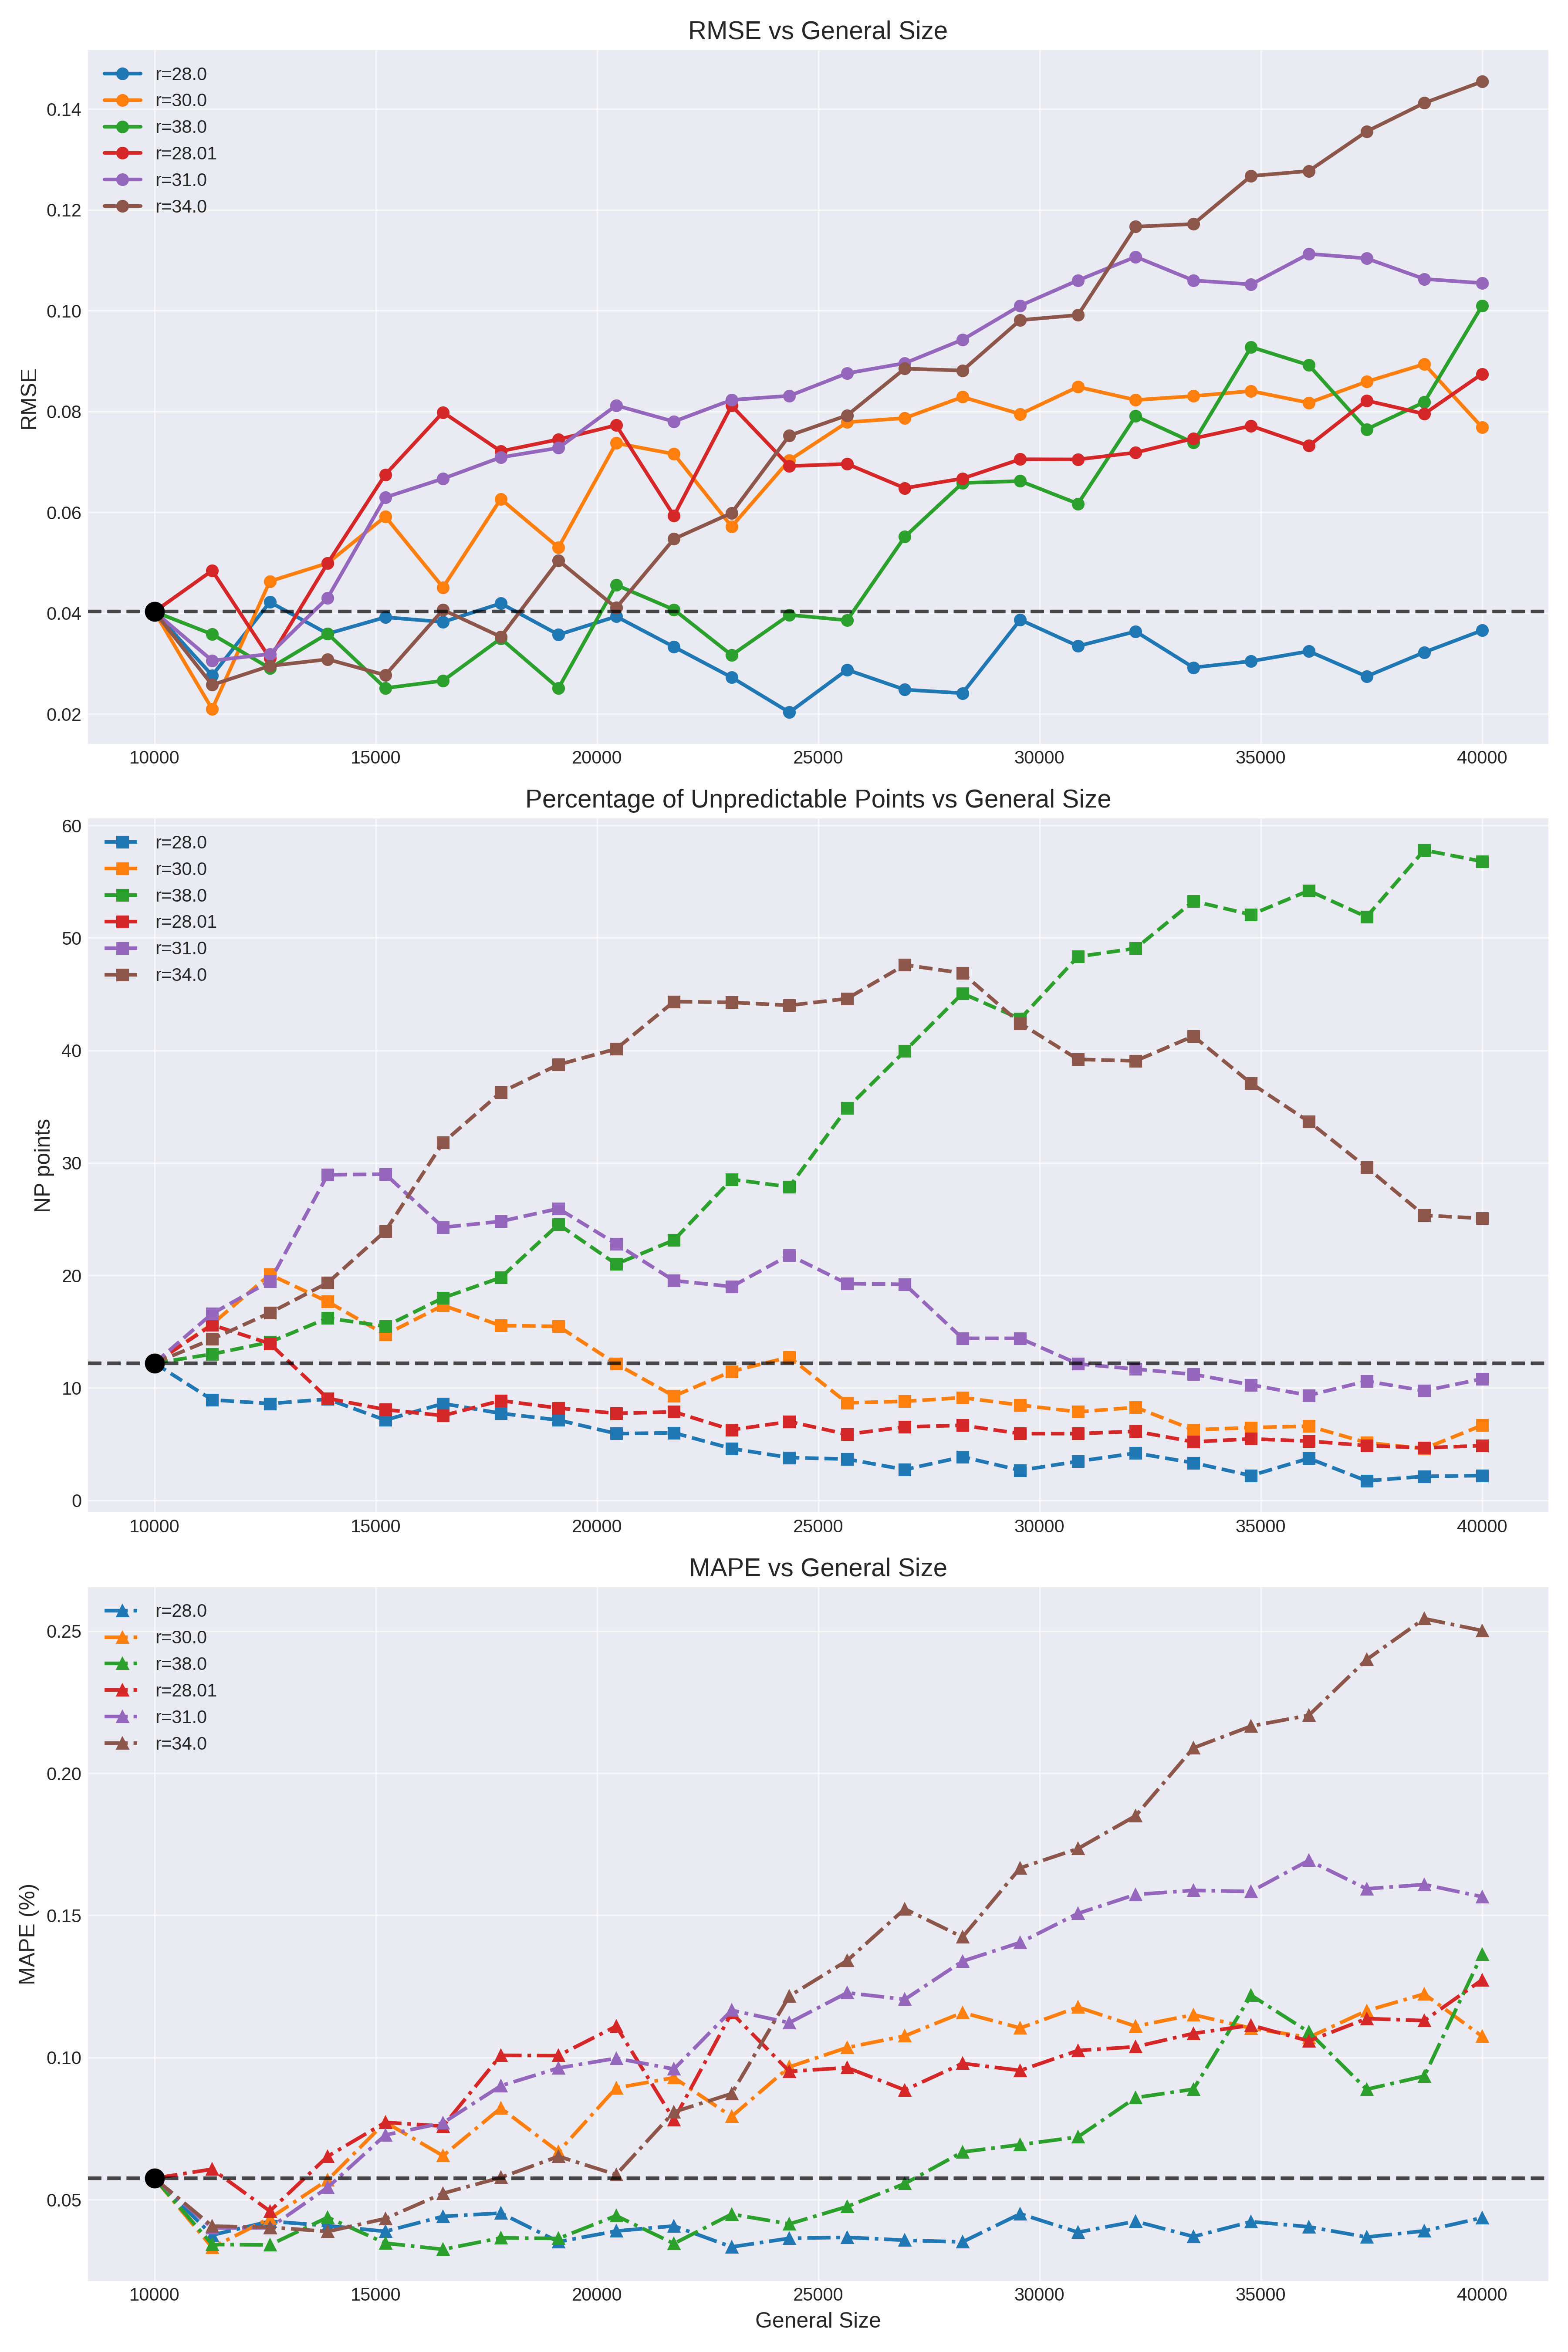
\includegraphics[width=0.8\textwidth]{../Size_experiment/unlucky_experiments.png}
    \caption{Зависимость метрик от суммарного размера обучающей выборки для
    случаев неэффективного расширения (r = 28.01, 31, 38, 34,31,30). }
    \label{fig:unlucky_exp}
\end{figure}

\paragraph{Анализ случаев ухудшения метрик (Рисунок \ref{fig:unlucky_exp}):}
 Когда параметр `r` вспомогательного ряда значительно отличался от базового,
  снижение количества непрогнозируемых точек происходило ценой резкого роста
   ошибок RMSE и MAPE. Это указывает на деградацию качества прогноза при
   смешивании данных из систем с существенно различной динамикой. Однако,
    не все случаи с близкими параметрами приводят к улучшению:
    например, при добавлении данных с r=28.01 предсказание не улучшается
     и остается на уровне базовой выборки из 10000 точек, без снижения MAPE или RMSE.
Также важен тот факт,что вне зависимости от выбора вспомогательного ряда,
  увеличение объема обучающей выборки всегда приводит к снижению доли
   непрогнозируемых точек при устремлении к бесконечности размера добавленного ряда.Это видно на примере 
   r = 34,r=31,r=30-со увеличением размера этих рядов в обучающей выборке
    число непрогнозируемых точек начинает снижаться.
     Это связано с тем,что со временем z-вектора добавленного ряда начинают 
   доминировать над z-векторами оригинального ряда.Но если  ряд близок по параметру, то новые z-вектора будут согласоваться
    с оригинальными,что видно на графиках \ref{fig:main_exp}  и \ref{fig:unlucky_exp},когда при добавлении небольшого 
    обьема выборки(5000 точек) против 10000 точек оригинального ряда,количество 
    непрогнозируемых точек начинает снижаться.
\subsection{Исследование зависимости эффекта аугментации от расхождения параметров.}
\subsubsection{Описание эксперимента}

Экспериментальная установка была определена следующим образом:
\begin{itemize}
    \item \textbf{Целевой ряд} \(Y^{(0)}\) был сгенерирован системой Лоренца с
     каноническим параметром \(r_0 = 28\).

    \item \textbf{Базовая обучающая выборка} \(\mathcal{D}_{\text{base}}\) была
     сформирована из первых \(N_{\text{base}} = 5000\) наблюдений целевого ряда:
    \[
    \mathcal{D}_{\text{base}} = \{y_0^{(0)}, y_1^{(0)}, \dots, y_{N_{\text{base}}-1}^{(0)}\}.
    \]

    \item \textbf{Вспомогательные ряды.} Был сгенерирован набор вспомогательных
     временных рядов \(\{Y^{(r)}\}\) для каждого значения параметра \(r\) из исследуемого множества \(\mathcal{R}\).

    \item \textbf{Гибридные обучающие выборки.} Для каждого \(r \in \mathcal{R}\)
     формировалась гибридная обучающая выборка \(\mathcal{D}_{\text{train}}^{(r)}\)
     путем объединения базовой выборки \(\mathcal{D}_{\text{base}}\) с сегментом из
     первых \(N_{\text{aux}} = 5000\) наблюдений соответствующего вспомогательного ряда \(Y^{(r)}\):
    \[
    \mathcal{D}_{\text{train}}^{(r)} = \mathcal{D}_{\text{base}} \cup \{y_0^{(r)},
     y_1^{(r)}, \dots, y_{N_{\text{aux}}-1}^{(r)}\}.
    \]
    Таким образом, для всех \(r\) размер гибридной выборки оставался постоянным: \(|\mathcal{D}_{\text{train}}^{(r)}| = N_{\text{base}} + N_{\text{aux}} = 10000\).

    \item \textbf{Оценка качества.} Для каждой выборки \(\mathcal{D}_{\text{train}}^{(r)}\)
     производилось прогнозирование на тестовом наборе данных (из ряда \(Y^{(0)}\)), и
      вычислялись значения функционалов качества: \(RMSE(r)\) ,\(MAPE(r)\) \(NP(r)\).
\end{itemize}

Результаты, представленные как функции от параметра \(r\), сравнивались с двумя контрольными уровнями:
\begin{enumerate}
    \item Качество прогноза на малой выборке, \(\text{RMSE}(\mathcal{D}_{\text{base}})\) и
     \(\text{NP}(\mathcal{D}_{\text{base}})\).
    \item Качество прогноза на «чистой» выборке эквивалентного размера, состоящей
     только из данных целевого ряда, \(\mathcal{D}_{\text{target\_large}} = \{y_0^{(0)}, \dots, y_{9999}^{(0)}\}\).
\end{enumerate}
\begin{figure}[htbp]
    \centering
    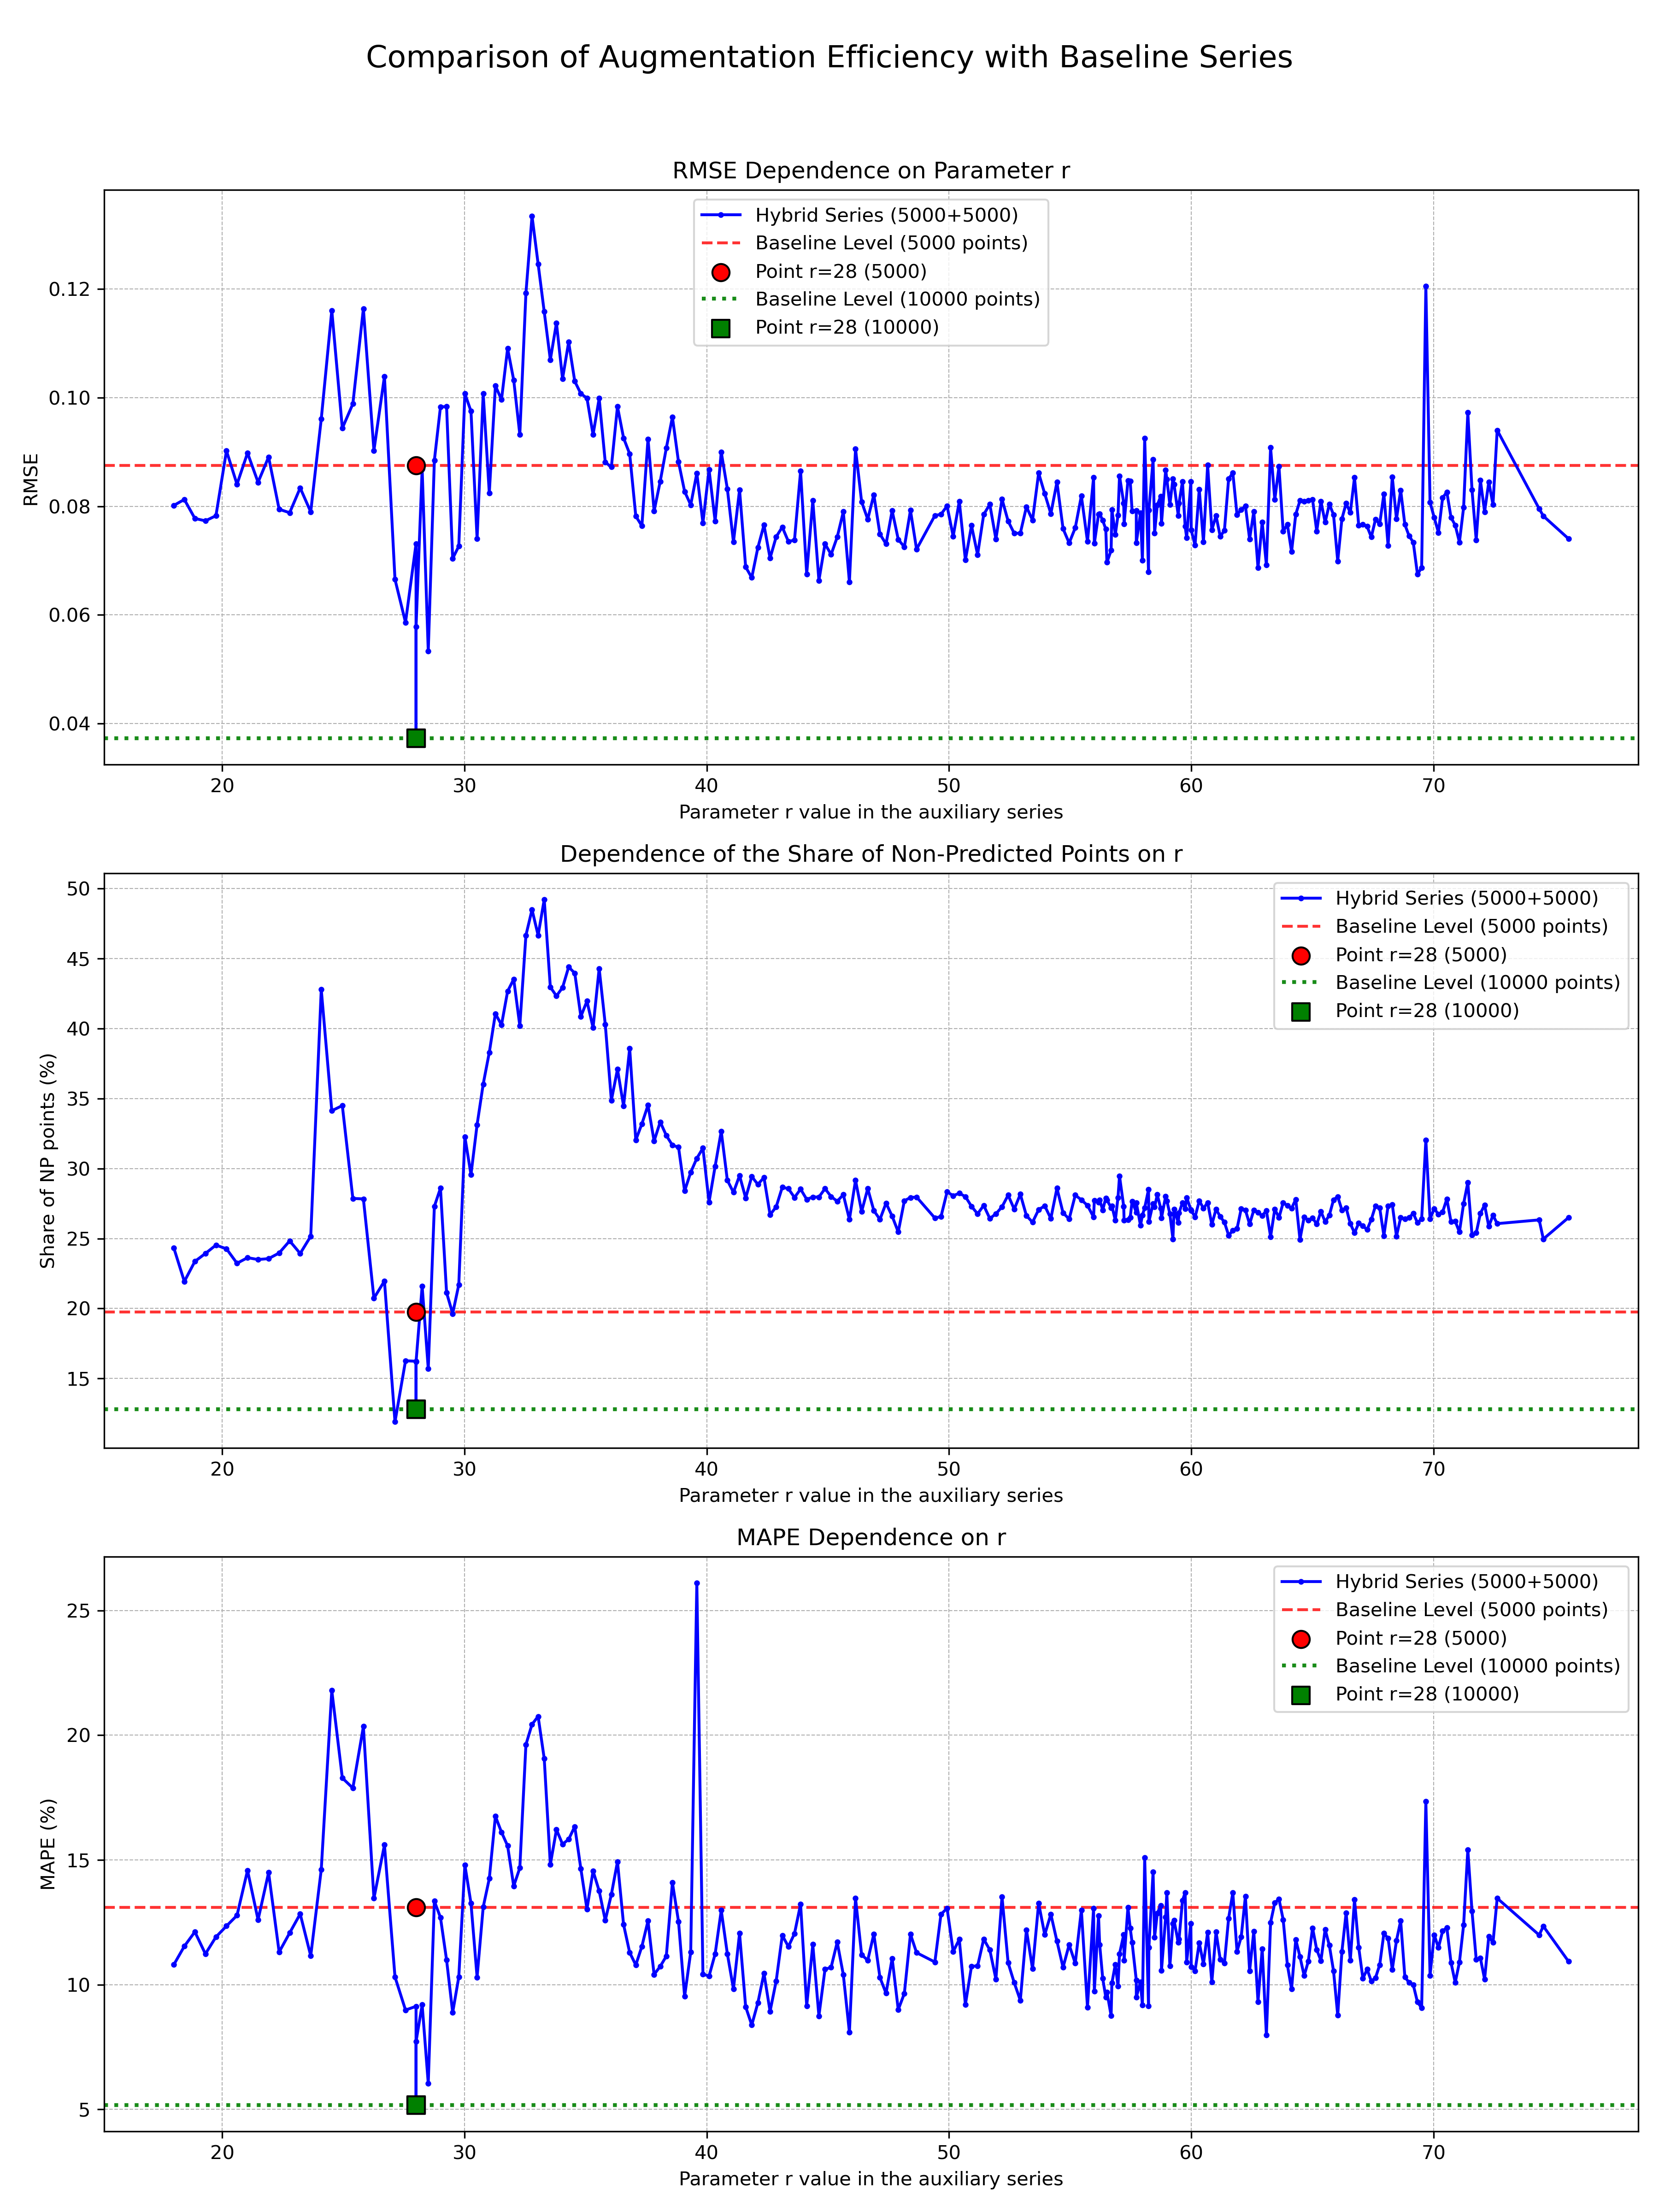
\includegraphics[width=0.8\textwidth]{../deviations/Different_r_comparison_with_points.png}
    \caption{Сравнение метрик при добавлении 5000 точек из ряда с различным
    параметром r к 5000 точкам основного ряда.}
    \label{fig:different_r}
\end{figure}
\subsubsection{Анализ эксперимента}

Результаты (Рисунок \ref{fig:different_r}) показывают, что существует узкая окрестность (26,30)
 вокруг `r=28`, в которой добавление вспомогательных рядов приводит к
  улучшению метрик по сравнению с базовой выборкой из 5000 точек. Эта окрестность
  никак не связана с бифуркационной картиной.
  В лучших случаях достигается снижение RMSE и NP в 1.5 раза.
   Однако даже в лучших случаях качество прогноза уступает результатам,
    полученным на выборке из 10000 точек исходного ряда.


\subsection{Разработка и валидация критерия отбора рядов-доноров}

\subsubsection{Описание эксперимента}
Предыдущие эксперименты показали, что не все формально близкие ряды одинаково
 полезны для аугментации. Это ставит задачу разработки критерия для априорной 
 оценки прогностической совместимости временных рядов. В данном эксперименте
  была проведена апробация метрики, основанной на сравнении статистических инвариантов
   динамики рядов, что тесно связано с методологией, представленной в работе Berardi et al. \cite{Berardi2018}.

\paragraph{Алгоритм вычисления метрики схожести.}
Теоретической основой для сравнения динамических систем служит \textbf{оператор Перрона-Фробениуса}, который описывает эволюцию плотностей вероятности состояний системы во времени. Поскольку аналитическое выражение для этого оператора в сложных системах недоступно, для его оценки применяется численный подход, заключающийся в построении \textbf{эмпирической матрицы вероятностей перехода}. Эта матрица является конечномерной аппроксимацией оператора Перрона-Фробениуса. Алгоритм ее построения и последующего сравнения состоит из следующих шагов:

\begin{enumerate}
    \item \textbf{Дискретизация фазового пространства.} Для корректного сравнения динамик оба временных ряда, эталонный $Y^{(1)}$ и ряд-кандидат $Y^{(2)}$, приводятся к дискретному представлению на общей сетке. Определяется глобальный диапазон амплитуд $[V_{\min}, V_{\max}]$, который затем разбивается на $K$ непересекающихся интервалов (состояний) $\{C_1, \dots, C_K\}$. В экспериментах использовалось $K=32$. Каждое непрерывное значение в рядах заменяется на номер состояния, в которое оно попадает, что приводит к формированию двух последовательностей дискретных состояний, $\mathcal{S}^{(1)}$ и $\mathcal{S}^{(2)}$.

    \item \textbf{Построение эмпирической матрицы перехода.} Для каждой дискретной последовательности $\mathcal{S}$ строится матрица $\mathbf{T}$ размером $K \times K$. Элемент $T_{ij}$ подсчитывает количество наблюдаемых переходов из состояния $C_i$ в состояние $C_j$ за один шаг по времени. Далее производится нормировка каждой строки матрицы на ее сумму. В результате матрица счетчиков преобразуется в стохастическую матрицу, элемент $T_{ij}$ которой оценивает условную вероятность перехода в состояние $j$ при условии нахождения в состоянии $i$. Эта матрица и является искомой конечномерной аппроксимацией оператора Перрона-Фробениуса.

    \item \textbf{Вычисление расхождения между операторами.} Схожесть двух динамических систем оценивается путем сравнения их матричных аппроксимаций оператора, $\mathbf{T}^{(1)}$ и $\mathbf{T}^{(2)}$. В качестве меры расхождения используется норма Фробениуса разности этих матриц:
    \[
    \mathcal{D}(Y^{(1)}, Y^{(2)}) = ||\mathbf{T}^{(1)} - \mathbf{T}^{(2)}||_F = \sqrt{\sum_{i=1}^{K}\sum_{j=1}^{K} (T_{ij}^{(1)} - T_{ij}^{(2)})^2}.
    \]
    Чем меньше значение этой нормы, тем ближе статистические свойства динамик двух систем, и тем более совместимыми они считаются для аугментации.
\end{enumerate}

\paragraph{Процедура эксперимента.}
С использованием описанной метрики была проведена следующая процедура:
\begin{itemize}
    \item Было сгенерировано 1000 вспомогательных рядов системы Лоренца, где управляющий
     параметр $r$ случайным образом варьировался в диапазоне $\pm 5$ от эталонного значения
      $r_0=28$ (т.е., $r \in [23, 33]$).
    \item Каждый из 1000 рядов-кандидатов был сравнен с эталонным рядом ($r=28$) с помощью
     описанной выше метрики. На основе полученных оценок были отобраны 47 рядов с наименьшим 
     значением нормы Фробениуса. Эта группа получила название \textbf{Отобранная аугментация}.
    \item Для контроля была сформирована вторая группа, \textbf{Случайная аугментация}, 
    в которую вошло 40 рядов, выбранных случайным образом из той же тысячи кандидатов.
    \item Для каждого ряда из обеих групп была сформирована гибридная обучающая выборка: 
    10,000 точек оригинального ряда ($r=28$) и 20,000 точек вспомогательного ряда.
    \item Качество прогноза для каждой гибридной выборки оценивалось по метрикам RMSE, 
    MAPE и доле непрогнозируемых точек.Подсчет метрик производился аналогично прошлым экспериментам,
    но для улучшения визуального эффекта был выбран другой гиперпараметр для идентификации
     непрогнозируемых точек.
\end{itemize}

\subsubsection{Анализ результатов}

\begin{figure}[htbp]
    \centering
    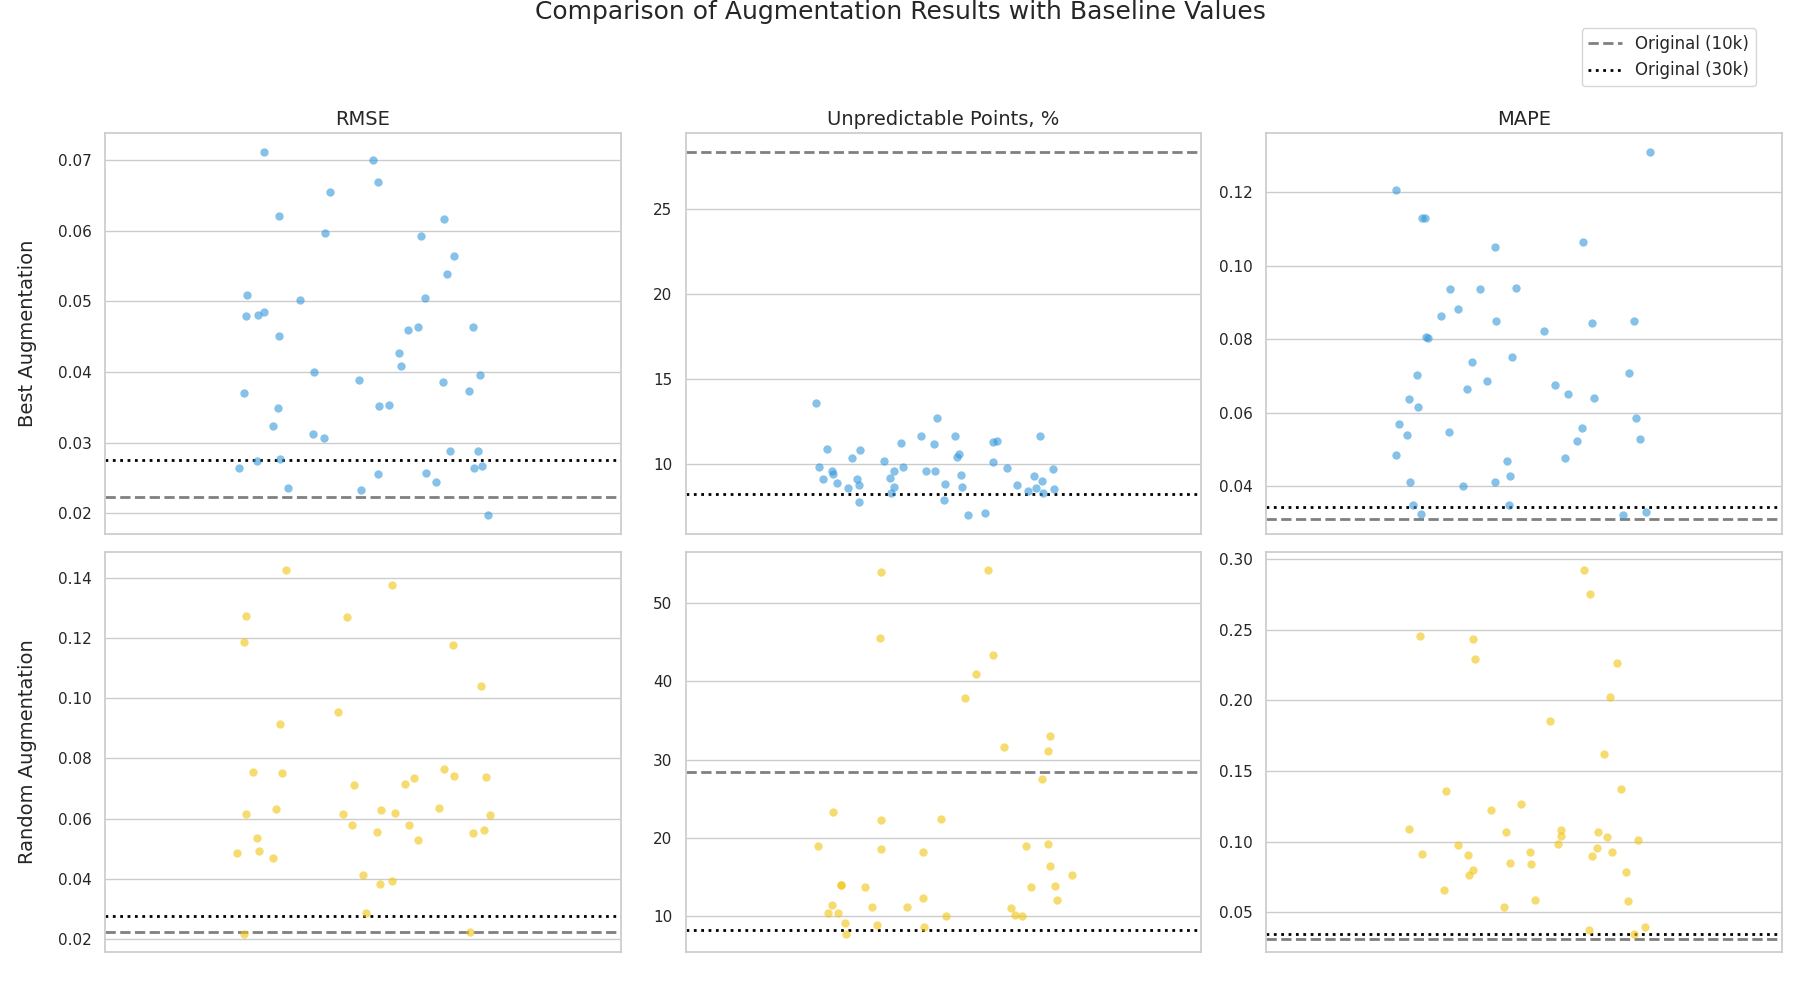
\includegraphics[width=\textwidth]{../mannayuitni/Augmentations_benefit_visualisation.png}
    \caption{Сравнение метрик качества прогноза для выборок, аугментированных отобранными
     (верхний ряд) и случайными (нижний ряд) рядами. Горизонтальные линии показывают эталонные
      уровни для выборок из 10,000 (пунктир) и 30,000 (точки) наблюдений оригинального ряда.}
    \label{fig:metric_validation}
\end{figure}

Результаты эксперимента, представленные на Рисунке~\ref{fig:metric_validation}, наглядно
 демонстрируют высокую эффективность предложенного критерия отбора. Визуально заметно, 
 что разброс значений метрик для отобранной группы значительно меньше, а сами значения в 
 среднем ниже (лучше), чем для случайной группы.

Это визуальное наблюдение находит строгое количественное подтверждение в результатах
 статистического анализа. Для сравнения распределений метрик между группами Отобранная 
 аугментация и Случайная аугментация был применен \textbf{критерий Манна-Уитни}. Тест
  показал, что по всем трем метрикам отобранная группа демонстрирует статистически значимо лучшие результаты:
\begin{itemize}
    \item \textbf{RMSE:}  p-значение $\approx 5.3 \times 10^{-7}$.
    \item \textbf{Nonpredictable points:} p-значение $\approx 9.1 \times 10^{-9}$.
    \item \textbf{MAPE:}  p-значение $\approx 1.4 \times 10^{-5}$.
\end{itemize}
Крайне низкие p-значения ($p \ll 0.001$) однозначно свидетельствуют о том, что 
предложенная метрика, основанная на сравнении численных аппроксимаций оператора Перрона-Фробениуса, успешно и неслучайно выделяет ряды, которые приводят к улучшению качества прогноза.

При детальном рассмотрении графиков видно, что максимальное значение RMSE для
 отобранных рядов не превышает 0.07, в то время как для случайных оно достигает
  вдвое больших значений. Аналогичная картина наблюдается и для метрики MAPE.
   Важно отметить, что для всех отобранных рядов доля непрогнозируемых точек сократилась как минимум вдвое по сравнению с исходной выборкой в 10,000 точек,
    при этом точность прогноза ухудшилась в большинстве случаев,но не более чем в два раза.

результаты эксперимента подтверждают, что предложенная метрика является
 эффективным инструментом отбора рядов-доноров для уменьшения числа непрогнозируемых точек.
 Более того, он открывает путь к дальнейшей оптимизации: очевидно, что если сделать 
 требования к метрике еще более строгими (например, ограничив ее сверху константой 
 так, чтобы выбирались 10 самых лучших из 1000 аугментаций), то можно будет получить
  качество прогноза, не уступающее идеальному случаю обучения на выборке из 30,000 
  точек оригинального ряда. Кроме того, существует зависимость между качеством аппроксимации 
  оператора и объемом исходных данных. Использование временных рядов большей длины позволяет
   увеличить размерность матрицы перехода при дискретизации пространства состояний, что, 
   в свою очередь, снижает погрешность аппроксимации оператора Перрона-Фробениуса.




\section{Заключение}

В данной работе было проведено исследование одной из фундаментальных проблем прогнозирования хаотических систем — дефицита данных для надежной реконструкции аттрактора. Была экспериментально проверена гипотеза о возможности восполнения этого дефицита за счет привлечения данных из схожих по динамике, но формально независимых систем.
Ключевым результатом работы стало выявление нетривиального характера 
прогностической совместимости временных рядов. Эксперименты показали, 
что положительный эффект от аугментации не гарантирован и зависит от
 сложной нелинейной согласованности динамик, а не от формальной близости 
 управляющих параметров. Пример с рядами при 
r=28.0001 и 
r=28.01 наглядно продемонстрировал несостоятельность стандартных метрик
 глобальной схожести и поставил задачу разработки более глубокого критерия отбора рядов-доноров.
Основным вкладом данной работы является предложение и апробация такого 
критерия, основанного на сравнении конечномерных аппроксимаций оператора 
Перрона-Фробениуса. Экспериментальная проверка подтвердила, что предложенная 
метрика является эффективным инструментом. Ряды, отобранные с ее помощью, показали 
статистически значимо лучшие результаты по сравнению со случайно выбранными, что
 подтверждено критерием Манна-Уитни. Однако важно подчеркнуть природу достигаемого улучшения: 
основной эффект заключается в существенном сокращении доли непрогнозируемых 
точек, что повышает "покрытие" и робастность прогноза. Это достигается 
ценой некоторого, как правило, контролируемого роста ошибки (RMSE, MAPE) 
на оставшихся прогнозируемыми точках. Таким образом, метрика позволяет не 
столько улучшить точность в абсолютном выражении, сколько избежать катастрофической
 деградации прогноза, характерной для неудачно подобранных рядов-доноров.
Таким образом, данное исследование предлагает не идеальное решение, а важный
 методологический шаг, позволяющий перейти от эмпирического подбора к 
 алгоритмическому отбору совместимых данных. Эксперименты на данных системы
  Лоренца показали, что действительно полезные ряды-доноры встречаются редко 
  (порядка 4 процентов от случайно сгенерированных в небольшом диапазоне), что подчеркивает практическую
   ценность предложенного фильтрующего механизма. Более того, точность самой метрики 
   зависит от длины анализируемых рядов, что является естественным ограничением. 
   Тем не менее, предложенный подход превращает метод межсерийного расширения данных 
   в управляемый и надежный инструмент для повышения полноты прогноза в условиях,
    когда получение длинных стационарных выборок невозможно. Это превращает
      метод межсерийного расширения данных в инструмент для достижения максимальной
       точности в условиях, когда получение длинных стационарных выборок невозможно,  что создает перспективы 
       для его применения в таких прикладных областях , как финансовые рынки, климатология,
 анализ биомедицинских сигналов или изучение паттернов энергопотребления \cite{PerezChacon2018}.
\section{Благодарности}
Проведение вычислительных экспериментов, описанных в данной работе, стало
 возможным благодаря использованию ресурсов Суперкомпьютерного комплекса НИУ ВШЭ.

\newpage
\printbibliography[title={Список использованных источников}]

\end{document}